\documentclass[DM,authoryear,toc]{lsstdoc}
\input{meta}
\graphicspath{{./}{figures/}}
\usepackage{amsmath}
% Package imports go here.

% Local commands go here.

%If you want glossaries
%\input{aglossary.tex}
%\makeglossaries

\title{Effects of Persistence and E2V Sensors using DC2 Data}

% Optional subtitle
% \setDocSubtitle{A subtitle}

\author{%
John Banovetz
}

\setDocRef{DMTN-276}
\setDocUpstreamLocation{\url{https://github.com/lsst-dm/dmtn-276}}

\date{\vcsDate}

% Optional: name of the document's curator
% \setDocCurator{The Curator of this Document}

\setDocAbstract{%
In this technote, I describe the process that I used to evaluate the effects persistence would have on the LSST survey. 
For this, I took persistence characterization values from electro-optical testing and modified raw DC2 images to include this model of persistence. 
I then ran the raw images through the DRP and analyzed the results. 
I found that the persistence adds a possibly non-negligible amount of flux to faint sources and can affect a significant amount of pixels. 
}

% Change history defined here.
% Order: oldest first.
% Fields: VERSION, DATE, DESCRIPTION, OWNER NAME.
% See LPM-51 for version number policy.
\setDocChangeRecord{%
  \addtohist{1}{YYYY-MM-DD}{Unreleased.}{John Banovetz}
}


\begin{document}

% Create the title page.
\maketitle
% Frequently for a technote we do not want a title page  uncomment this to remove the title page and changelog.
% use \mkshorttitle to remove the extra pages

% ADD CONTENT HERE
% You can also use the \input command to include several content files.

\section{Camera Level Persistence}
Persistence was first found in Run 5 of electro-optical (EO) testing at SLAC. Further investigation found that this effect only affected E2V sensors. 
This persistence was found to have an average signal after the flash of 6 ADU and had a decay constant of 37 seconds. 
It was also foud that the persistence only went away with integration time. One of the unique features of this persistence is the persistence trail. 
Not only do the saturated pixels have an increased signal, but so do all the pixels leading to the end of the amplifier in the parallel direction.


\section{Effect of Persistence on DC2 Images}

\begin{figure*}[!htp]
  \centering
  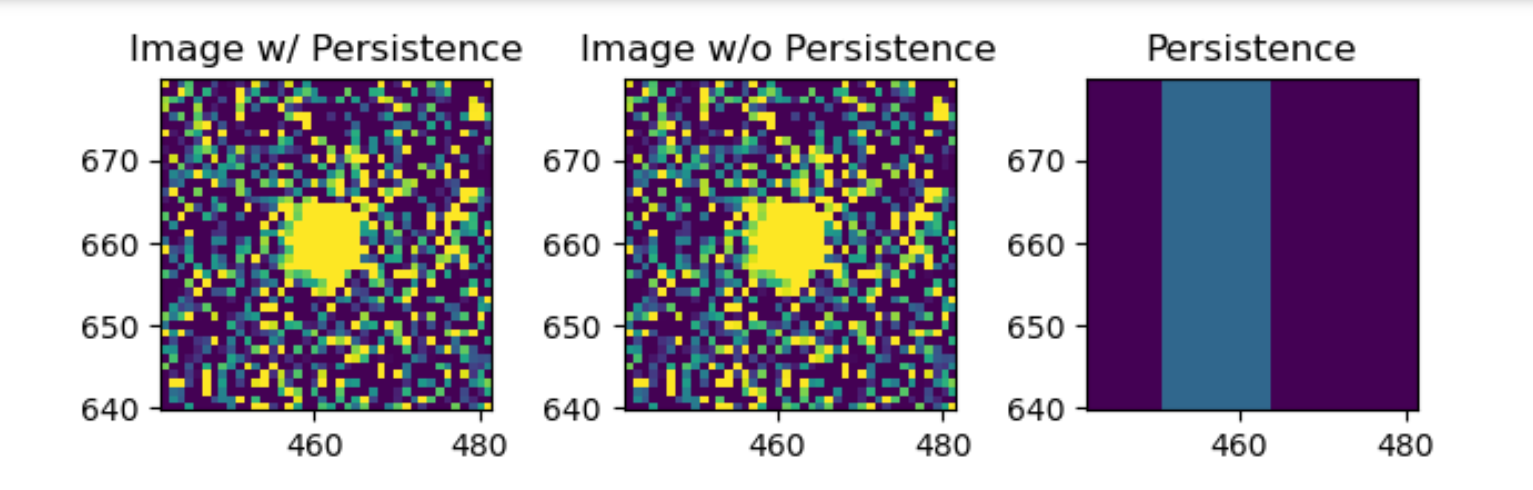
\includegraphics[width=0.95\textwidth, angle=0]{Obj_pers.png}
  \caption{
  A zoomed in object that shows the persistence affected image (left), the original image (middle) 
  and the subtraction between the two to highlight the persistence (right).
  }\label{fig:ex_persistence}
\end{figure*}

\begin{figure*}[!htp]
  \centering
  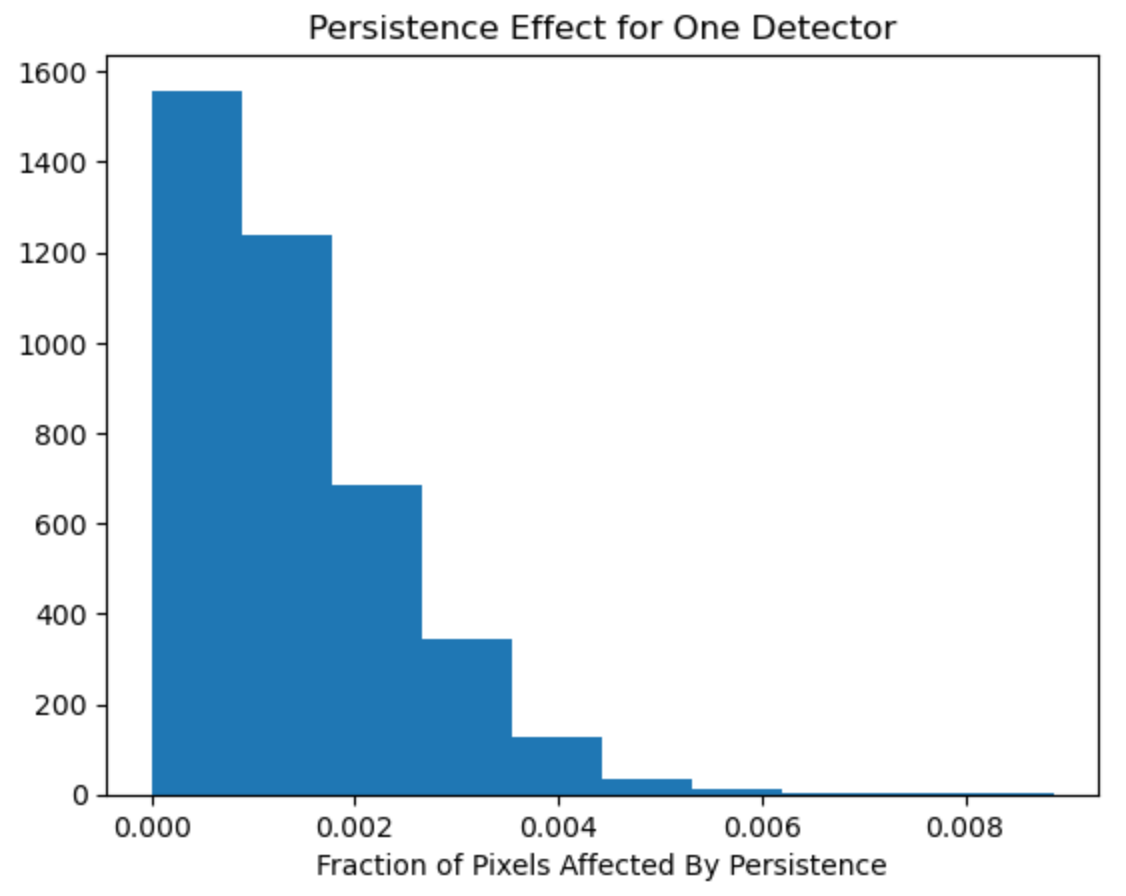
\includegraphics[width=0.95\textwidth, angle=0]{DC2_percent_affected_pixels.png}
  \caption{
  The percentage of affected pixels using 4000 sequential DC2 images. The majority of the images have $<0.2\%$ of their pixels affected. 
  }\label{fig:affected_pixels}
\end{figure*}


Since this effect will not be easily removed, I looked into how persistence will affect LSST like images and measurements on the objects. 
I adopted the same model as desribed above for the persistence and its trail and added it into subsquent images. 
Figure \ref{fig:ex_persistence} shows an example of a DC2 image and the model persistence applied to it. 
I then plotted a histogram of the fraction of persistence affected pixels as seen in Figure \ref{fig:affected_pixels}. 
This shows the number of images with the corresponidng fraction of affected pixels. 
For most images, $<0.2\%$ of pixels are affected in the subsquent images.


\section{Effect of Persistence on DC2 Objects}

\begin{figure*}[!htp]
  \centering
  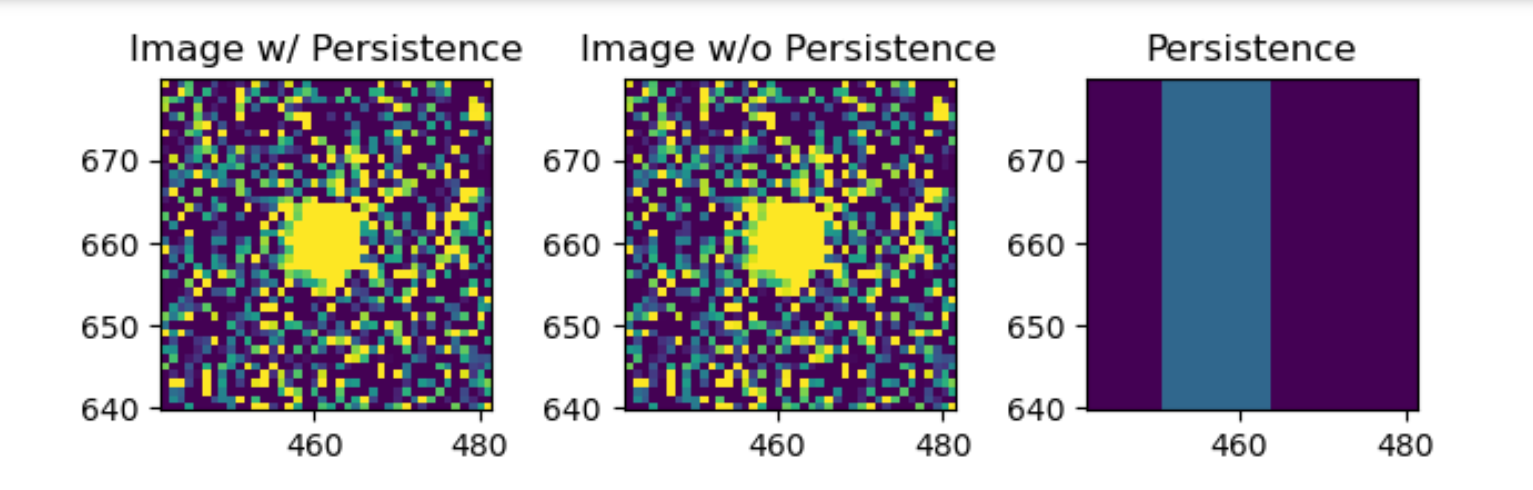
\includegraphics[width=0.95\textwidth, angle=0]{Obj_pers.png}
  \caption{
  A zoomed in object that shows the persistence affected image (left), the original image (middle) 
  and the subtraction between the two to highlight the persistencet (right)
  }\label{fig:obj_persistence}
\end{figure*}

To measure the effect that this would have on DC2 objects, I used a small subset of data (around 20 images) from DC2 
found in this collection \texttt{$`2.2i/runs/test-med-1/w_2023_17/DM-39092'$}. 
Taking the raw images from this dataset, 
I ran a similar process to the procedure in measuring the effect on an a suite of DC2 images and added the persistence in. 
I then saved these images as \texttt{$`raw_modified'$} images and ran these types of images through the DRP pipeline up until the 'calexp' image step.
These images can be found in the collection \texttt{$`u/banovetz/dc2/w_2023_34/raw_persistence_single_value_output'$}

There were roughly 200 objects in these 20 images that were affected by persistence an example of which can be seen in Figure \ref{fig:obj_persistence}.
Comparing these objects with and without persistence, 
I found that those with persistence would have a difference of magnitude of about 0.001-0.01 magnitude for those dimmer than ~19-20 magnitude. 
Figure \ref{fig:absolute_fractional_flux} shows the fractional magnitude difference between the persistence affected images and the originals
 as a function of magnitude ordered objects (with 0 being the brightest object).

\begin{figure*}[!htp]
  \centering
  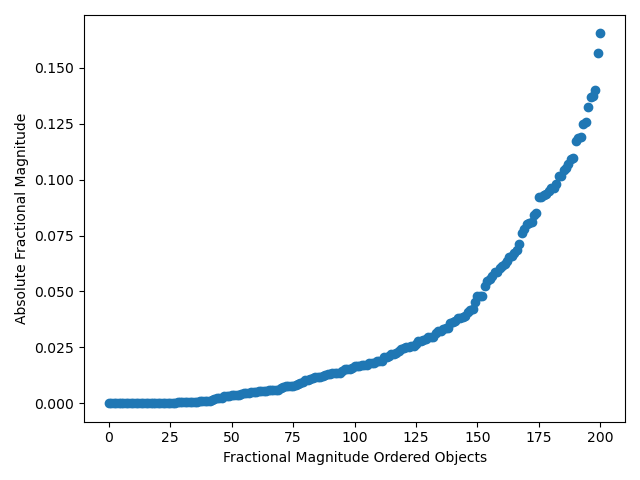
\includegraphics[width=0.95\textwidth, angle=0]{Absolute_Fractional_Magnitude.png}
  \caption{
  A zoomed in object that shows the persistence affected image (left), the original image (middle) 
  and the subtraction between the two to highlight the persistencet (right)
  }\label{fig:absolute_fractional_flux}
\end{figure*}

This can be explained as these objects have an area of roughtly 100 square pixels and the trails caused by the persisence can be 10--20 pixels wide.
Increase the flux by 100--600 ADU of an object would cause this discrepancy.


\appendix
% Include all the relevant bib files.
% https://lsst-texmf.lsst.io/lsstdoc.html#bibliographies
\section{References} \label{sec:bib}
\renewcommand{\refname}{} % Suppress default Bibliography section
\bibliography{local,lsst,lsst-dm,refs_ads,refs,books}

% Make sure lsst-texmf/bin/generateAcronyms.py is in your path
\section{Acronyms} \label{sec:acronyms}
\addtocounter{table}{-1}
\begin{longtable}{p{0.145\textwidth}p{0.8\textwidth}}\hline
\textbf{Acronym} & \textbf{Description}  \\\hline

DM & Data Management \\\hline
\end{longtable}

% If you want glossary uncomment below -- comment out the two lines above
%\printglossaries





\end{document}
